  

\section{Joachimsthal's Integral}

\textcolor{red}{ron: introduzir e uniformizar notacao}


\begin{proposition}\label{prop:invariant_joachim} Consider an ellipse $\mathcal{E}$ defined by $\langle A P,P\rangle=1$. Let $u$ be an inward unit vector in the direction of the billiard orbit passing through the point $P_0\in\mathcal{E} $. Let $T(P_1,u)=(P_2,v)$ the billiard map as shown in   \cref{fig:appC-joachim}.
	Then 
	\[  \langle A P_1,u\rangle =  -\langle A P_2,u\rangle=  \langle A P_2,v\rangle  \]
\label{prop:appA-joachim}
	\end{proposition}

%trim=left bottom right top
\begin{figure}[H]
	\begin{center}
 %	\def\svgwidth{0.75\textwidth}
	 %	\input{pics_tex/joachim.eps_tex}
	 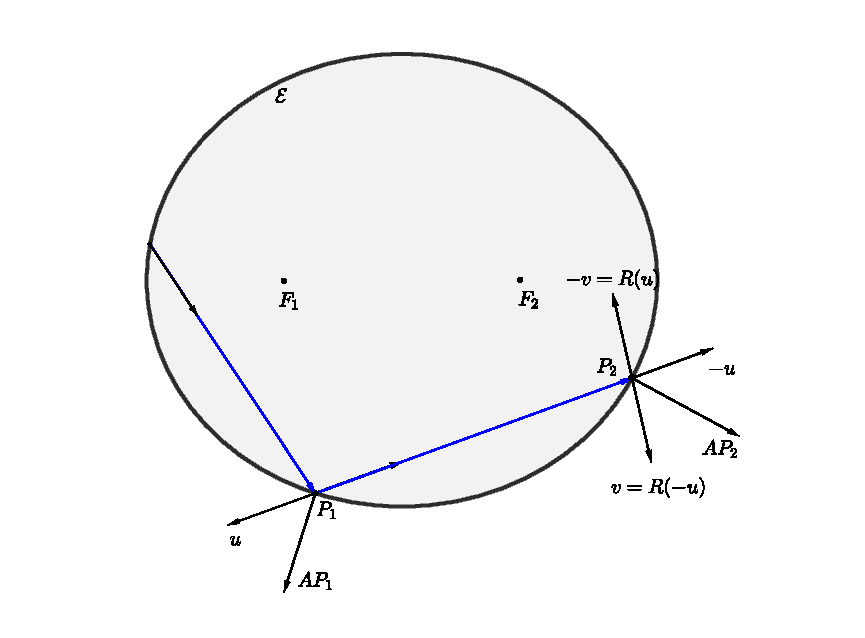
\includegraphics[scale=0.6]{pics_appC_050_joachimstall.pdf}
	 %	 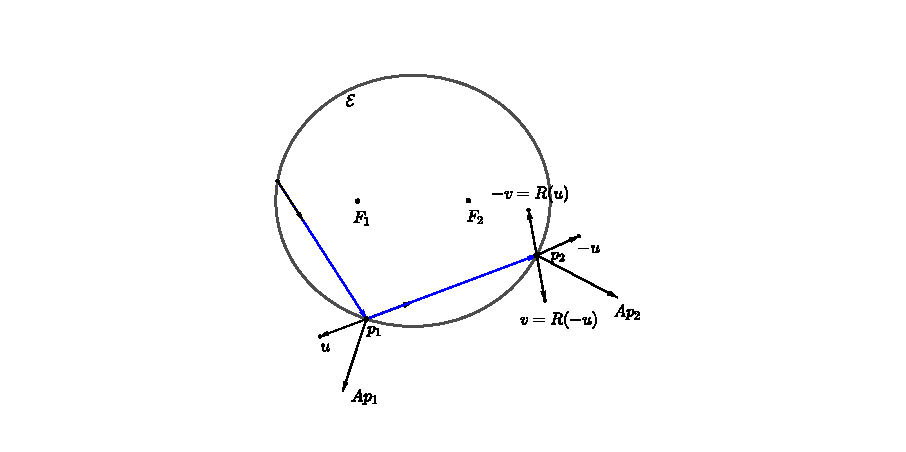
\includegraphics[scale=0.9]{pics_tex/joachimstall.pdf}
		\caption {Joachimsthal's first integral  $\langle AP_1,u\rangle $ is T-invariant.}
		 \label{fig:appC-joachim}
	\end{center}
\end{figure}

\begin{proof} The tangent space  $T_{p}\mathcal{E}$ is formed of the vectors $u$ such that $ \langle A P,u\rangle =0.$ Therefore $AP$ is a normal vector to the ellipse at the point $P$. The vector $u$ is proportional to $P_2-P_1$.
	
	Therefore,
	\begin{align*}  \langle AP_1+AP_2 , P_2-P_1\rangle &= \langle AP_1  , P_2 \rangle + \langle AP_2  , P_1 \rangle  - \langle AP_1  , P_1 \rangle + \langle AP_2  , P_2 \rangle \\
	&= \langle  P_1  , AP_2 \rangle - \langle AP_2  , P_1 \rangle =0. 
	\end{align*}
	Then,
	\[ \langle AP_1 , u\rangle =\langle  AP_2 ,-u\rangle  =  \langle  AP_2 ,R(-u)\rangle  =  \langle  AP_2, v\rangle \]
	\end{proof}
	
	\begin{proposition}
	    In a confocal pair of ellipses
	    \[\mathcal{E}:\; \frac{x^2}{a^2}+\frac{y^2}{b^2}=1,\;\; \mathcal{E}_c:\; \frac{x^2}{a_c^2}+\frac{y^2}{b_c^2}=1\]
	    it follows that
	   \[ J  =\frac{\sqrt{  a^2 - a_c^2}}{a b} \]
	      \label{prop:appA-confocal-EE}
	\end{proposition}
	
	\begin{proof} Follows directly from \cref{prop:appA-joachim}.
	    
	\end{proof}
	
	\begin{proposition}
	    In a confocal pair of conics
	    \[\mathcal{E}:\; \frac{x^2}{a^2}+\frac{y^2}{b^2}=1,\;\; \mathcal{H}_c:\; \frac{x^2}{a_c^2}-\frac{y^2}{b_c^2}=1\]
	    it follows that
	     \[ J  =\frac{\sqrt{  a^2 - a_c^2}}{a b} \]
	    \label{prop:appA-confocal-EH}
	\end{proposition}
	
	\begin{proof}
	    In this case we  recall that $c^2=a^2-b^2=a_c^2+b_c^2$
	\end{proof}
	
	\begin{proposition}
	    Consider an ellipse $\E$ with semi-axes $a$ and $b$ \textrm{(}$a>b$\textrm{)} and a billiard orbit with Joachimstall's invariant $J$.
	    If $0<J<1/a$ \textrm{(}resp. $1/b> J> 1/a$\textrm{)} the caustic is an ellipse (resp. an hyperbola).
	\end{proposition}
	
	\begin{proof} Consider the point $P_1=[0,b].$ It follows that
	$J=\sin\theta/b$, where $\theta$ is the angle of the segment of orbit  $P_1P_2$  with the tangent vector $(-1,0)$. This orbit pass through the focus $F_1=[-c,0]$ when $\sin\theta=b/a$. So the result follows since the caustic is   hyperbolic or elliptic when the segment $P_1P_2$ intersects the focal segment $F_1F_2$ or not.  
	    
	\end{proof}